\section{Risks - placeholder} \label{risks}
\subsection{Mark Allocation}

v. \textbf{Risks -- 10\%}

\textit{list specific risks and show how you deal with them}

\subsection{Detail Task Description} 

v. develop a risk register that identifies risks, their likelihood, potential impact and mitigation strategies;

\subsection{Proposal Structure}

A risk register, documenting risks, their likelihood and impact, and procedures that will be put in place to mitigate against these risks and recover from them should they occur. A table is usually considered to be the best way to present this information concisely.

Markers will consider whether: a risk register has been completed along with impacts and mitigation strategies; the key risks are identified and compared in terms of likelihood and impact; listed risks are project specific, credible and show breadth of thinking in terms of risk source and type; it is clear how risks will be managed; mitigation strategies are appropriate and effective; innovation and pragmatism are evident.

\subsection{Another subsection}

Risk table goes here.

\textbf{Example of figure reference: see Figure \ref{fig:example}}. 
\lipsum[5]

\begin{figure}[ht]
\centering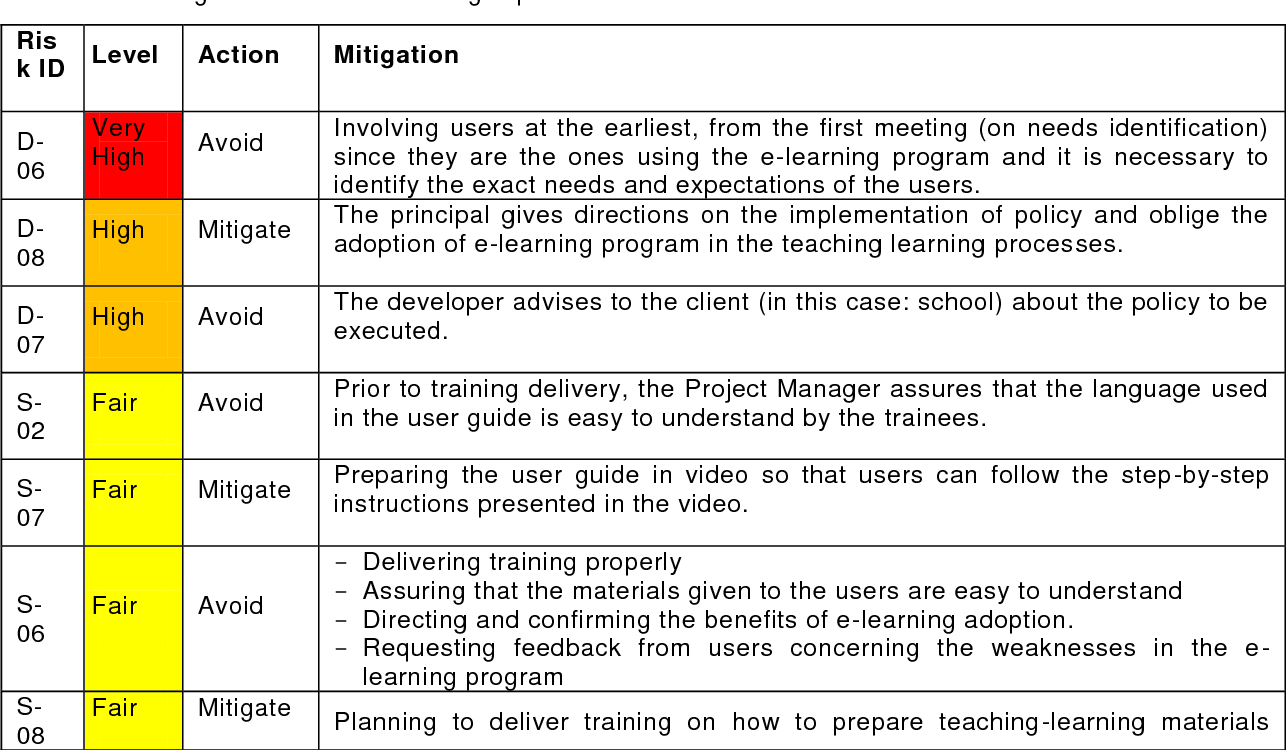
\includegraphics[width=1\linewidth]{risk-mitigation-table.png}
\caption{Risk mitigation table - might want to keep this to 5 items at most ~ 25\% of text height}
\label{fig:example}
\end{figure}

\textbf{Example of equation reference: see Equation \eqref{eq:emc}}. 
\lipsum[6]

\begin{equation} 
\label{eq:emc}
e = mc^2
\end{equation}

\subsection{Subsection 3}

\textbf{Example of reference to Section \ref{risks}.} 
\lipsum[7]
\lipsum[8]